\documentclass[12pt]{article}
%\usepackage{helvet}
%\renewcommand{\familydefault}{\sfdefault}
\usepackage{amsfonts}
\usepackage{amsmath}
\usepackage{amssymb}
\usepackage{bm}
\usepackage{fullpage}
\usepackage{setspace}
\usepackage{graphicx}
\usepackage{gensymb}
\usepackage[nottoc,numbib]{tocbibind}
\usepackage{graphicx}
\usepackage{float}
\usepackage{braket}
\usepackage{titlesec}
\usepackage{siunitx}
\usepackage{mathtools}
\usepackage{tikz}
\usepackage[font={small}]{caption}
\usepackage{subcaption}
\usepackage[inline]{enumitem}
%\titlespacing*{\section}{0pt}{4pt}{4pt}
\usepackage[letterpaper, margin=2cm]{geometry}


\begin{document}
\pagenumbering{arabic}
\spacing{1.5}

%%%%%%%%%%%
% Begin Document
%%%%%%%%%%%

\section{Free energy}
In it's most general form, the free energy of a material which is composed of chiral, rod-like molecules, and has a crystalline density structure is given by the free energy
\begin{align}\label{eq:Fgeneral}
\mathcal{F} = \int_{\mathrm{all\:space}}d^3r\left(f(Q_{ij},\partial_kQ_{lm},\phi)+g(\nabla_{\parallel}\phi,\nabla_{\bot}\phi)+h(\phi)\right),
\end{align}
where $Q_{ij}$ is the (tensor) order parameter, which is spatially non-uniform and non-zero in any non-isotropic phase, and $\phi$ is the density order parameter which quantifies the change in density from some reference phase, $\rho_{ref}$ (which is homogeneous in density). There are two pieces to this free energy:
\begin{enumerate}[label=\roman*]
	\item The liquid crystal free energy, $f(Q_{ij},\partial_kQ_{lm},\phi)$, which penalizes any non-equilibrium distortions (e.g. splay, bend, twist) in the average molecular orientation.
	\item The phase-field crystal free energy, $g(\nabla_{\parallel}\phi,\nabla_{\bot}\phi)$, which in general allows for periodic modulations in the density below some transition temperature, $T_m$. $\nabla$ is broken up into it's parallel and perpendicular components with respect to the local orientation of the rod-like molecules. A potential well term, $h(\phi)$, which encourages non-zero $\phi$ values below some transition temperature $T_p$ (which could in general be different than $T_m$) is also included.
\end{enumerate}

\subsection{Liquid crystal free energy}
In what follows, I will make several large assumptions in the form of the first term in eqn \ref{eq:Fgeneral}.
\begin{enumerate}[label=1.\alph*]
\item The first assumption concerns the liquid crystal free energy term, and in particular the order parameter $Q_{ij}$. Although we are interested in modelling chiral (collagen) molecules, I will assume that the biaxiality of the molecules is small so we are in the "low chirality limit" \cite{Wright:1989zz}. In this limit, $Q_{ij}$ is uniaxial, and can be written as
\begin{align}\label{eq:simpleQ}
Q_{ij}=\lambda(3n_in_j-\delta_{ij}),
\end{align}
where $\lambda$ is a position-dependent quantity related to the usual uniaxial scalar order parameter $S(r)=1/2\left<3cos^2\theta-1\right>$, and $n_i$ are the components of the director field $\bm{n}(\bm{r})$ which gives the average, local molecular orientation. Since a uniaxial $Q_{ij}$ tends to minimize the bulk (gradient-less) components of the liquid crystal free energy, we ignore these terms in our system, and consider only the deformation free energy, which for uniaxial liquid crystals can most recognizably be written in the form
\begin{align}
f_{\mathrm{frank}}(\nabla\bm{n})=&\frac{1}{2}\hat{K}_{11}(\nabla\cdot\bm{n})^2+\frac{1}{2}\hat{K}_{22}(\bm{n}\cdot\nabla\times\bm{n}+q)^2+\frac{1}{2}\hat{K}_{33}(\bm{n}\times(\nabla\times\bm{n}))^2\nonumber\\
&+\hat{k}_{13}\nabla\cdot(\nabla\cdot\bm{n})\bm{n}-\frac{1}{2}(\hat{K}_{22}+\hat{k}_{24})\nabla\cdot(\bm{n}\times(\nabla\times\bm{n})+\bm{n}(\nabla\cdot\bm{n}))
\end{align}
where I have assumed $\lambda$ is constant and absorbed it into the definitions of the elastic constants $\hat{K}_{ii}$ and $\hat{k}_{ij}$.

\item Since we are interested in modelling collagen fibril structure, I am going to assume that the liquid crystal material is constrained to be within a cylinder of radius $R$ and infinite length, and so the elastic constants are essentially zero outside of the cylinder (as it is surrounded by some isotropic fluid). This changes the domain of integration from all of space to just that of the cylinder. This also has the consequence that the divergence terms (preceded by the elastic constants $\hat{k}_{13}$ and $\hat{K}_{22}+\hat{k}_{24}$) cannot be neglected, and introduces an interfacial free energy per unit length $\mathcal{F}_s/L=2\pi\gamma R$. This assumption is justified as long as the interactions between individual rod-like molecules and the surrounding isotropic fluid cause the molecules to aggregate, which we will take to be true. Furthermore, with this assumption we are neglecting interactions between cylinders, although these interactions could perhaps be modelled using some sort of coarse-grained defect interaction term $\sim\ln(R/|x_j-x_i|)$ \cite{Chaikin:318158}, where $|x_j-x_i|$ is the distance between cylinders.

\item The director field is constrained to be that of a double-twist structure, with $\bm{n}=\sin\psi(r)\hat{\theta}+\cos\psi(r)\hat{z}$ (potential error in here with a minus sign in the $\hat{\theta}$ term\footnote{any change in sign of this term will just correspond to a redefinition of the sign of the inverse pitch $q$, which we in the end will fix anyway to match up with the right-handedness of the fibrils}).

\item The density modulations $\phi$ are small enough perturbations as to not affect the values of the elastic constants within the cylinder. Thus, to first order the liquid crystal free energy does not depend on $\phi$.
\end{enumerate}

Thus, integrating over the first integral in equation \ref{eq:Fgeneral} with the above assumptions,
\begin{align}
\int_{\mathrm{all\:space}}d^3rf(Q_{ij},\partial_kQ_{lm},\phi)&=2\pi L\int_0^{\infty}rdr f_{\mathrm{frank}}(\nabla\bm{n}_{\mathrm{double-twist}})\nonumber\\
&=2\pi L\int_0^{R}rdr\left(\frac{1}{2}K_{22}\left(q-\psi'-\frac{\sin2\psi}{2r}\right)^2+\frac{1}{2}K_{33}\frac{\sin^4\psi}{r^2}\right)\nonumber\\
&\phantom{=}-\pi L(K_{22}+k_{24})\sin^2\psi(R)+2\pi\gamma R L.
\end{align}

\subsection{Phase field crystal free energy}
The most general terms obeying the symmetries of the rod-like molecules for the second term in eqn \ref{eq:Fgeneral} is
\begin{align}
g(\nabla_{\parallel}\phi,\nabla_{\bot}\phi)=-a_{\parallel}(\nabla_{\parallel}\phi)^2+b_{\parallel}(\nabla_{\parallel}^2\phi)^2-a_{\bot}(\nabla_{\bot}\phi)^2+b_{\bot}(\nabla_{\bot}^2\phi)^2+c(\nabla_{\parallel}\phi)^2(\nabla_{\bot}\phi)^2.
\end{align}
For thermodynamic stability, both $b_{\parallel}>0$ and $b_{\bot}>0$. $a_{\parallel}$ and $a_{\bot}$ can be of either sign in principle, and should change sign according to some transition temperature $T_m$.\footnote{It could be possible that there are two transition temperatures, one for ordering parallel to the molecules, and a second for ordering perpendicular to the molecules.}

To ensure that non-zero density amplitude modulations are thermodynamically favourable, we also include the third term in eqn \ref{eq:Fgeneral}, which can most simply be written as
\begin{align}
h(\phi)=d\phi^2(e\phi^2-1).
\end{align}

The simplifying assumptions I make to reduce the number of terms in the above two equations are:
\begin{enumerate}[label=2.\alph*]
\item \label{asspfc:1} The local density modulations perpendicular to the rod-like molecules are unimportant and can be coarse-grained out of the free energy, so that I can set any terms containing $\nabla_{\bot}$ to $0$. For collagen fibrils in particular, this ignores the hexagonal-like packing of molecules within the fibril, which occur over length scales of $\approx\SI{1}{\nano\meter}$.
\item \label{asspfc:2} The density modulations only occur along the axis of the cylinder, so $\phi(\bm{r})\to\phi(z)$. This axis is in general not along the average local direction of the molecules ($\hat{z}\neq\bm{n}$).
\item \label{asspfc:3} The density modulations have a well defined period, which I will call $\eta$. This allows us to average over a period of the structure.
\end{enumerate}

The definitions of $\nabla_{\parallel}$ and $\nabla_{\bot}$ are given in terms of the local coordinates of the average orientation of molecules $\bm{x}^{\prime}$, which I define with respect to the lab reference frame $\bm{x}$. The transformation $\bm{x}^{\prime}=A\bm{x}$ written explicitly is
\begin{align}
\begin{bmatrix}
	x^{\prime}+r \\
	y^{\prime} \\
	z^{\prime}.
\end{bmatrix}
=
\begin{bmatrix}
	\cos\theta			&\sin\theta			& 0\\
	-\sin\theta\cos\psi(r)	&\cos\theta\cos\psi(r)	&-\sin\psi(r)\\
	-\sin\theta\sin\psi(r)	&\cos\theta\sin\psi(r)		&\cos\psi(r)
\end{bmatrix}
\begin{bmatrix}
	x \\
	y \\
	z
\end{bmatrix}
\end{align}
and the inverse transformation is
\begin{align}
\begin{bmatrix}
	x \\
	y \\
	z
\end{bmatrix}
=
\begin{bmatrix}
	\cos\theta			&-\sin\theta\cos\psi(r)	& -\sin\theta\sin\psi(r)\\
	\sin\theta			&\cos\theta\cos\psi(r)	&\cos\theta\sin\psi(r)\\
	0				&-\sin\psi(r)			&\cos\psi(r)
\end{bmatrix}
\begin{bmatrix}
	x^{\prime}+r \\
	y^{\prime} \\
	z^{\prime}.
\end{bmatrix}.
\end{align}
The geometry of this local coordinate system is illustrated in Figure \ref{fig:coordinates}. Importantly, $\theta$ and $r$ (and so $\psi(r)$) are held constant in this definition, and should not be thought of as functions of $x$ and $y$ when defining local derivatives $\nabla_{\parallel}$ and $\nabla_{\bot}$.

\begin{figure}[t]
	\centering
	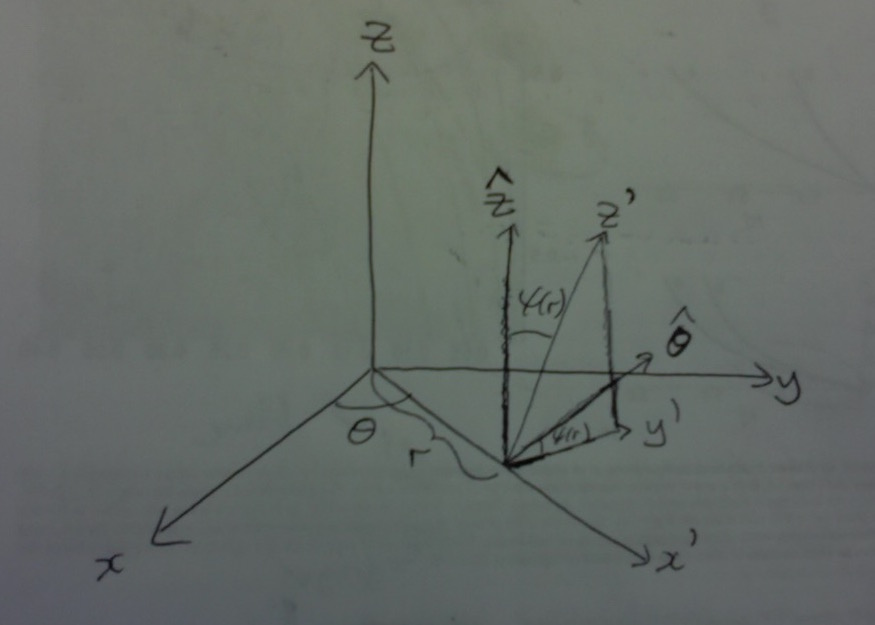
\includegraphics[width=0.5\textwidth]{{figures/coordinates}.jpg}
	\caption{Defining the local (primed) coordinates of the average molecular orientation with respect to the lab reference frame.}\label{fig:coordinates}
\end{figure}

With these transformations, I can define more concretely the gradient
\begin{align}
\nabla_{\parallel}&=\hat{z}^{\prime}\frac{\partial}{\partial z^{\prime}}\nonumber\\
&=\hat{z}^{\prime}\left(-\sin\theta\sin\psi(r)\frac{\partial}{\partial x}+\cos\theta\sin\psi(r)\frac{\partial}{\partial y}+\cos\psi(r)\frac{\partial}{\partial z}\right),
\end{align}
With assumption \ref{asspfc:1}, I don't need to evaluate $\nabla_{\bot}$, but I will for completeness as it draws attention to the fact that $\partial/\partial z$ terms exist in $\nabla_{\bot}$, so both assumptions \ref{asspfc:1} and \ref{asspfc:2} are required to safely ignore any $\nabla_{\bot}$ terms, as
\begin{align}
\nabla_{\bot}&=\hat{x}^{\prime}\frac{\partial}{\partial x^{\prime}}+\hat{y}^{\prime}\frac{\partial}{\partial y^{\prime}}\nonumber\\
&=\hat{x}^{\prime}\left(\cos\theta\frac{\partial}{\partial x}+\sin\theta\frac{\partial}{\partial y}\right)+\hat{y}^{\prime}\left(-\sin\theta\cos\psi(r)\frac{\partial}{\partial x}+\cos\theta\cos\psi(r)\frac{\partial}{\partial y}-\sin\theta\frac{\partial}{\partial z}\right).
\end{align}

Using assumptions \ref{asspfc:1} and \ref{asspfc:2} and the identities $(\nabla\phi)^2=\nabla\cdot(\phi\nabla\phi)-\phi\nabla^2\phi$ and $(\nabla^2\phi)^2=\nabla\cdot\nabla(\phi\nabla^2\phi)-2\nabla\cdot(\phi\nabla\nabla^2\phi)+\phi\nabla^4\phi$, I can re-write the phase field crystal parts of the free energy as
\begin{align}\label{eq:pfc1}
\int_{\mathrm{all\:space}}d^3rg(\nabla_{\parallel}\phi,\nabla_{\bot}\phi)&=2\pi\frac{\Lambda}{2}\int_0^Rrdr\int_0^{\frac{2\pi}{\eta}}dz\phi(z)\left(\left(\frac{2\pi}{d_{\parallel}}\right)^2+cos^2\psi(r)\frac{\partial^2}{\partial z^2}\right)^2\phi(z)+\mathcal{F}_{surf},
\end{align}
\begin{align}
\int_{\mathrm{all\:space}}d^3rh(\phi)=\omega\pi R^2\int_0^{\frac{2\pi}{\eta}}dz\left(\frac{\phi(z)}{\chi}\right)^2\left(\left(\frac{\phi(z)}{\chi}\right)^2-1\right).
\end{align}
The terms $\mathcal{F}_{surf}$ are obtained through integration by parts, and in general cannot be neglected for the same reasons that the divergence terms in the frank free energy cannot be neglected. However, since all of these terms are integrated through a dot product of $\hat{d\bm{S}}=\hat{r}$ and some vector with direction $\hat{\bm{V}}=\hat{\nabla\phi}=\hat{z}$ by assumption \ref{asspfc:2}, they are zero in our case. I have also taken the free parameter $\chi^2>0$, which is not necessary in general. $\chi^2>0$ is equivalent physically to only looking at our system below the critical temperature where density modulations occur (which is where we are interested in investigating). The parameter $d_{\parallel}$ is just the preferred period of the density modulations, and will in general not be equivalent to the true period $\eta$ because of the $\cos^2\psi(r)$ term in eqn \ref{eq:pfc1}.

\subsection{Final form of the free energy per unit volume}
In this section, I will use hats to denote dimensional variables, and no hats as dimensionless variables. For the dimensional case, I can write the free energy per fibril volume ($\pi R^2 2\pi/\eta$) bulk phase (i.e. array) of cylindrical, liquid crystalline collagen fibrils as
\begin{align}
\hat{E}(\hat{R},\hat{\eta};\hat{\psi}(\hat{r}),\hat{\phi}(\hat{z}))&=\frac{2}{\hat{R}^2}\int_0^{\hat{R}}\hat{r}d\hat{r}\left(\frac{1}{2}\hat{K}_{22}\left(\hat{q}-\hat{\psi}'-\frac{\sin2\hat{\psi}}{2\hat{r}}\right)^2+\frac{1}{2}\hat{K}_{33}\frac{\sin^4\hat{\psi}}{\hat{r}^2}\right)\nonumber\\
&\phantom{=}+\frac{\hat{\Lambda}\hat{\chi}^2}{\hat{R}^22\pi/\hat{\eta}}\int_0^{\hat{R}}\hat{r}d\hat{r}\int_0^{\frac{2\pi}{\hat{\eta}}}d\hat{z}\:\frac{\hat{\phi}(\hat{z})}{\hat{\chi}}\left(\left(\frac{2\pi}{\hat{d}_{\parallel}}\right)^2+cos^2\hat{\psi}(\hat{r})\frac{\partial^2}{\partial \hat{z}^2}\right)^2\!\!\frac{\hat{\phi}(\hat{z})}{\hat{\chi}}\nonumber\\
&\phantom{=}+\frac{\hat{\omega}}{2\pi/\hat{\eta}}\int_0^{\frac{2\pi}{\hat{\eta}}}d\hat{z}\left(\frac{\hat{\phi}(\hat{z})}{\hat{\chi}}\right)^2\left(\left(\frac{\hat{\phi}(\hat{z})}{\hat{\chi}}\right)^2-1\right)\nonumber\\
&\phantom{=}-(\hat{K}_{22}+\hat{k}_{24})\frac{\sin^2\hat{\psi}(\hat{R})}{\hat{R}^2}+\frac{2\hat{\gamma}}{\hat{R}^2}.
\end{align}

Note that the reason we are interested in the free energy per fibril volume instead of the total free energy, is that we assume the fibril phase has already been minimized with respect to volume $V_f=N_f\pi R^2 L$, and since the total free energy is
\begin{align}
\mathcal{F}&=N_f\pi \hat{R}^2\hat{L}\hat{E}\nonumber\\
&=V_f\hat{E},
\end{align}
we need to find the minimum of $\mathcal{F}$ with $V_f$ held constant.

If I take a single mode approximation for the density, $\hat{\phi}(\hat{z})=\hat{\delta}\cos(\hat{\eta}\hat{z})$ and replace all variables with their dimensionless forms
\begin{align}
&E=\frac{\hat{E}}{\hat{K}_{22}\hat{q}^2},\\
&R=\hat{R}\hat{q},\\
&r=\hat{r}\hat{q},\\
&\psi(r)=\hat{\psi}(\hat{r}),\\
&K_{33}=\frac{\hat{K}_{33}}{\hat{K}_{22}},\\
&L=\frac{\hat{L}}{\hat{d}_{\parallel}},\\
&\Lambda=\frac{\hat{\Lambda}\hat{\chi}^2}{\hat{K}_{22}\hat{q}^2\hat{d}_{\parallel}^4},\label{eq:dimensionlessLambda}\\
&\rho_{\delta}=\frac{\hat{\rho}_{\delta}}{\hat{\chi}},\\
&\delta=\frac{\hat{\delta}}{\hat{\chi}},\\
&\eta=\hat{\eta}\hat{d}_{\parallel},\\
&\omega=\frac{\hat{\omega}\hat{\chi}^4}{\hat{K}_{22}\hat{q}^2},\label{eq:dimensionlessomega}\\
&\gamma=\frac{\hat{\gamma}}{\hat{K}_{22}\hat{q}}.
\end{align}
then this becomes
\begin{align}\label{eq:finalE}
E(R,\eta,\delta;\psi(r))&=\frac{2}{R^2}\int_0^{R}rdr\left(\frac{1}{2}\left(1-\psi'-\frac{\sin2\psi}{2r}\right)^2+\frac{1}{2}K_{33}\frac{\sin^4\psi}{r^2}\right)\nonumber\\
&\phantom{=}+\frac{\Lambda\delta^2}{2R^2}\int_0^Rrdr\left(4\pi^2-\eta^2\cos^2\psi(r)\right)^2\nonumber\\
&\phantom{=}+\frac{\omega\delta^2}{2}\left(\frac{3}{4}\delta^2-1\right)-(1+k_{24})\frac{\sin^2\psi(R)}{R^2}+\frac{2\gamma}{R}.
\end{align}

\subsection{Free energy per fibril volume minimization}
To minimize eqn \ref{eq:finalE}, I start by taking
\begin{align}
\frac{\delta E}{\delta \psi}=0
\end{align}
which gives the differential equation
\begin{subequations}
\begin{align}\label{eq:psiODE}
\frac{d\psi}{dr}+r\frac{d^2\psi}{dr^2}=&1-\cos(2\psi)\left(1-\frac{\sin(2\psi)}{2r}\right)+K_{33}\frac{\sin(2\psi)\sin^2\psi}{r}\nonumber\\
&+\Lambda\delta^2\eta^2r(4\pi^2-\eta^2\cos^2\psi)\cos\psi\sin\psi,\\
\psi(0)=&0,\label{eq:psiBC0}\\
\frac{d\psi}{dr}\bigg|_{r=R}=&1+k_{24}\frac{\sin(2\psi(R))}{2R}.\label{eq:psiBCR}
\end{align}
\end{subequations}

To solve eqn \ref{eq:psiODE} with the boundary condition eqns \ref{eq:psiBC0} and \ref{eq:psiBCR}, I use an ODE numerical relaxation technique \cite{numrec}. I'm putting the equations below just for my own reference, where I'm letting $y_1=\psi(r)$ and $y_2=d\psi/dr$. The discretization goes has $M+1$ points, on the evenly spaced grid $r_1,...,r_{M+1}$ with spacing $h$.
\begin{subequations}
\begin{align}
E_{1,k}&=y_{1,k}-y_{1,k-1}-h\frac{(y_{2,k}+y_{2,k-1})}{2},\\
E_{1,M+1}&=y_{2,M}-1-k_{24}\frac{\sin(2y_{1,M})}{2r_M},\\
E_{2,k}&=y_{2,k}-y_{2,k-1}\nonumber\\
&\phantom{=}-\frac{2h}{r_k+r_{k-1}}\bigg\{1-\frac{(y_{2,k}+y_{2,k-1})}{2}-\cos(y_{1,k}+y_{1,k-1})\bigg(1-\frac{\sin(y_{1,k}+y_{1,k-1})}{r_k+r_{k-1}}\bigg)\nonumber\\
&\phantom{=-\frac{2h}{r_k+r_{k-1}}\bigg\{\}}+2K_{33}\frac{\sin^2\big((y_{1,k}+y_{1,k-1})/2\big)\sin(y_{1,k}+y_{1,k-1})}{r_k+r_{k-1}}\nonumber\\
&\phantom{=-\frac{2h}{r_k+r_{k-1}}\bigg\{\}}+\frac{\Lambda\delta^2\eta^2(r_k+r_{k-1})}{2}\big(4\pi^2-\eta^2\cos^2\big((y_{1,k}+y_{1,k-1})/2\big)\big)\nonumber\\
&\phantom{=-\frac{2h}{r_k+r_{k-1}}\bigg\{\}\Lambda\delta^2\eta^2(r_k+r_{k-1})}\cdot\cos\big((y_{1,k}+y_{1,k-1})/2\big)\sin\big((y_{1,k}+y_{1,k-1})/2\big)\bigg\},\\
E_{2,1}&=y_{1,1}
\end{align}
\end{subequations}
Taking the derivatives of these, I get for $k=2,...,M$
\begin{subequations}
\begin{align}
S_{1,1}&=-1,\\
S_{1,2}&=\frac{-h}{2},\\
S_{1,3}&=1,\\
S_{1,4}&=\frac{-h}{2},\\
S_{2,1}&=\frac{-2h}{r_k+r_{k-1}}\bigg\{\frac{2K_{33}}{r_k+r_{k-1}}\bigg(\frac{1}{2}\sin^2(y_{1,k}+y_{1,k-1})+\sin^2\big((y_{1,k}+y_{1,k-1})/2\big)\cos(y_{1,k}+y_{1,k-1})\bigg)\nonumber\\
&\phantom{=\frac{-2h}{r_k+r_{k-1}}\bigg\{\}}+\sin(y_{1,k}+y_{1,k-1})\bigg(1-\frac{\sin(y_{1,k}+y_{1,k-1})}{r_k+r_{k-1}}\bigg)+\frac{\cos^2(y_{1,k}+y_{1,k-1})}{r_k+r_{k-1}}\nonumber\\
&\phantom{=\frac{-2h}{r_k+r_{k-1}}\bigg\{\}}+\frac{\Lambda\delta^2\eta^2(r_k+r_{k-1})}{2}\bigg(\eta^2\cos^2\big((y_{1,k}+y_{1,k-1})/2\big)\sin^2\big((y_{1,k}+y_{1,k-1})/2\big)\nonumber\\
&\phantom{=\frac{-2h}{r_k+r_{k-1}}\bigg\{\}+\frac{\Lambda\delta^2\eta^2(r_k+r_{k-1})}{2}\bigg()}+\frac{1}{2}\big(4\pi^2-\eta^2\cos^2\big((y_{1,k}+y_{1,k-1})/2\big)\big)\nonumber\\
&\phantom{=\frac{-2h}{r_k+r_{k-1}}\bigg\{\}+\frac{\Lambda\delta^2\eta^2(r_k+r_{k-1})}{2}\bigg()}\cdot\big(\cos^2\big((y_{1,k}+y_{1,k-1})/2\big)-\sin^2\big((y_{1,k}+y_{1,k-1})/2\big)\big)\bigg)\bigg\},\\
S_{2,2}&=-1+\frac{h}{r_k+r_{k-1}},\\
S_{2,3}&=S_{2,1},\\
S_{2,4}&=1+\frac{h}{r_k+r_{k-1}}.
\end{align}
\end{subequations}
At the first boundary $k=1$ (corresponding to $r=0$), I get
\begin{subequations}
\begin{align}
S_{2,1}&=0,\\
S_{2,2}&=0,\\
S_{2,3}&=1,\\
S_{2,4}&=0.
\end{align}
and at the second boundary $k=M+1$ (corresponding to $r=R$), I get
\begin{align}
S_{1,1}&=0,\\
S_{1,2}&=1,\\
S_{1,3}&=-k_{24}\frac{\cos(2y_{1,M})}{r_M},\\
S_{1,4}&=1.
\end{align}
\end{subequations}

%%%%%%%%%%%%%%%
% Bibliography
%%%%%%%%%%%%%%%
\clearpage
\bibliography{pfc}
\bibliographystyle{unsrt}

\end{document}
